\section*{Bernoülli's Differential Equation}
A differential equation of form $y'+p(x) y=Q(x) y^{n} . n \in \mathbb{R} /\{0,1\}$ called Bernocilli's Differential equation

Method to solve:

i.) Divide by $y^{n}$

$$
	y^{-n} \cdot y'+p(x) y^{1-n}=Q(x)-(1)
$$

\begin{enumerate}
	\setcounter{enumi}{1}
	\item put $z \leq y^{1-n}, \therefore \frac{d z}{d x}=(1-n) y^{-n} \cdot \frac{d y}{d x} \Rightarrow \underbrace{y^{-n} \cdot \frac{d y}{d x}=\frac{1}{1-n} \cdot \frac{d z}{d x}}_{\text{(2) }}$

	\item Substitute (2) in (1):

\end{enumerate}

$(1) \rightarrow \frac{1}{1-n} \cdot \frac{d z}{d x}+P(x) \cdot z=Q(x)$

$$
	\Rightarrow z'+(1-n) P(x) \cdot z=(1-n) Q(x)
$$

This is FLDE. in dependent variable $z$

$\therefore$ Solution:

$$
	Z \cdot(I \cdot F)=\int(1-n) Q(x) \cdot I F \cdot d x+C \quad, I F=e^{\int(1-n) \cdot P(x) \cdot d x}
$$

Solve following:

a) $y'+2 y=y^2$

A. Divide by $y^2$ :

$$
	y^{-2} \cdot y'+2 y^{-1}=1
$$

put $z=y^{-1} \quad \therefore z \frac{d z}{d x}=-y^{-2} \cdot \frac{d y}{d x}$

$\therefore$ (1) becomes:

$-\frac{d z}{d x}+2 z=1 \Rightarrow \frac{d z}{d x}-2 x=-1$

This is FLDE.

$\therefore P(x)=-2, \quad Q(x)=-1$

$I F=e^{\int P d x}=e^{\int-2 \cdot d x}=e^{-2 x}$

$\therefore$ General Solution:

$$
	\begin{gathered}
		\therefore z \cdot e^{-2 x}=\int-e^{-2 x} d z+c / 2 \\
		z x e^{-2 x}=\frac{1}{2} e^{-2 x}+\frac{c}{2} \\
		\text{ now } z=y^{-1} \\
		\therefore \quad y^{-1} \cdot e^{-2 x}=\frac{1}{2} e^{-2 x}+\frac{c}{2} \\
		\therefore y=\frac{2}{1+e^{2 x} \cdot c}
	\end{gathered}
$$

Divide by $y^{4}$ :

$$
	y^{-4} \cdot \frac{d y}{d x}-y^{-3} \cdot \tan(x)=\sec (x)-(1)
$$

let $z=y^{-3}, \quad \frac{d z}{d x}=-3 . y^{-4} \cdot \frac{d y}{d x}$

multiply $\theta$ by -3 \& substitute $\frac{d z}{d x}$

$$
	+3, \quad z \tan(x)=-3 \sec (x)
$$

\begin{flalign*}
	 & \frac{d z}{d x}                                                                                      \\
	 & P(x)=3 \tan(x) \quad Q(x)=-3 \sec (x)                                                                \\
	 & I: F=e^{\int P \cdot d x}=e^{3 \int \tan x \cdot d x}=e^{\ln \left(\sec ^{3}(x)\right)}=\sec ^{3}(x)
\end{flalign*}

multiply (2) by I.F.

$\sec ^{3}(x) \cdot \frac{d z}{d x}+3 \cdot \tan(x) \cdot \sec ^{3}(x) z=-3 \sec ^{4}(x)$

Apply reverse product rule: $u v'+v u'=(4 v)'$

$$
	\Rightarrow \frac{d}{d x}\left(\sec ^{3}(x) \cdot z\right)=-3 \sec ^{4}(x)
$$

$\int s c .^{4} \rightarrow \int \operatorname{se}^{2} \cdot \operatorname{sc}^{2}$

Integrate both sides: $\rightarrow\left(1+t^{2}\right) s c^{2}$


\begin{equation*}
	\sec ^{3}(x) \cdot z=-3 \int \sec ^{4}(x) \cdot d x+c \tag{x}
\end{equation*}


$=\int(1+\infty) dt$

$$
	=-3\left[\tan(x)+\frac{\tan ^{3}(x)}{3}\right]+c
$$

$\Rightarrow \frac{\sec ^{3}(x)}{y^{3}}=-3 \tan(x)=\tan ^{3}(x)+c$

$\therefore y=\frac{1}{\operatorname{sos}^{5}(x) \cdot \sqrt[3]{-3 \tan(x)-\tan ^{3}(x)+c}}$

d) $\frac{d y}{d x}+\tan(x) \tan(y)=\cos(x) \cdot \sec (y)$

A) This is B.D.E.

Divide by $\sec (y)$

$\cos(y) \frac{d y}{d x}+\tan(x) \sin(y)=\cos(x) \quad-(1)$

let $z=\sin(y) . \quad \frac{d z}{d x}=\cos(y) \cdot \frac{d y}{d x}$.

Substitute this in (1)

$\frac{d z}{d x}+\tan(x) \cdot z=\cos(x)$

let IF $=e^{\int \tan(x) \cdot d x}=e^{\ln (\sec (z))}=\sec (x)$

multiply both sides by T.F.

$\sec (x) \cdot \frac{d z}{d x}+\tan(x) \cdot \sec (x) \cdot z \cdot=1$

$\equiv \frac{d}{d x}(\sec (x) \cdot z)=1 \quad \Rightarrow \quad \sec (x) \cdot z=x+c \Rightarrow \sec (x) \cdot \sin(y)=x+c$.

$\therefore y=\sin ^{-1}(\cos(x) \cdot(x+c))$\\
d) $\frac{d y}{d x}+x \cdot \sin(2 y)=x^{3} \cdot \cos ^{2}(y)$

Divide by $\cos ^{2}(y)$ :

$\sec ^{2}(y) \cdot \frac{d y}{d x}+\frac{x \cdot 2 \sin(y) \cos(y)}{\cos ^{2}(y)}=x^{3}$

$\sec ^{2}(y) \frac{d y}{d x}+2 x \cdot \tan(y)=x^{3} \quad-10$

let $z=\tan(y) \quad \frac{d y}{d x}=\sec ^{2}(y) \cdot \frac{d y}{d x}$

substitute this in (1):

$\frac{d z}{d x}+2 x \cdot z=x^{3}$\\
let I.F $e^{\sqrt{2 x} \cdot d x}=e^{x^2 }$, demultiply both sides by I.F $e^{x^2 } \cdot \frac{d z}{d x}+z \cdot 2 x \cdot e^{x^2 }=x^{3} e^{x^2 }$

$\Rightarrow \frac{d}{d x}\left(e^{x^2 } \cdot z\right)=x^{3} \varepsilon e^{x^2 }$

\begin{center}
	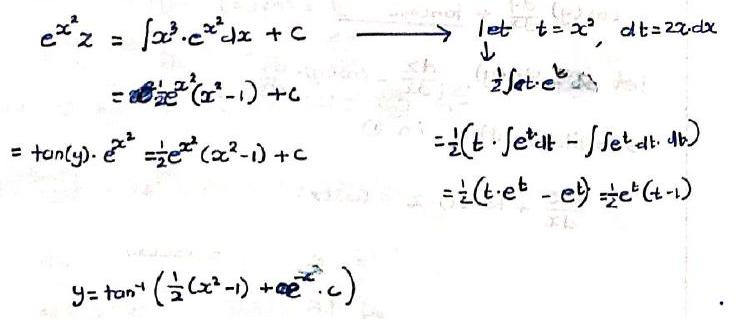
\includegraphics[max width=\textwidth]{2024_07_21_6c823ced6a9d46a245adg-4}
\end{center}

\section*{1.) $\frac{d y}{d x}+y=x y^{3} \quad$ 2) $\frac{d y}{d x}-y \tan(x)=y^2 \cdot \sec (x)$ \\
3) $\frac{d y}{d x}+\frac{y}{x}=\frac{y^2}{x} \ln (x)$ \\
4) $\frac{d y}{d x}+x y=x^{3} y^{3}$}
